% A simple figure to illustrate Mike and Frank's embedding
% Sept 2013

\documentclass{article}
\usepackage{tikz}

\begin{document}

\begin{figure}
\begin{center}
  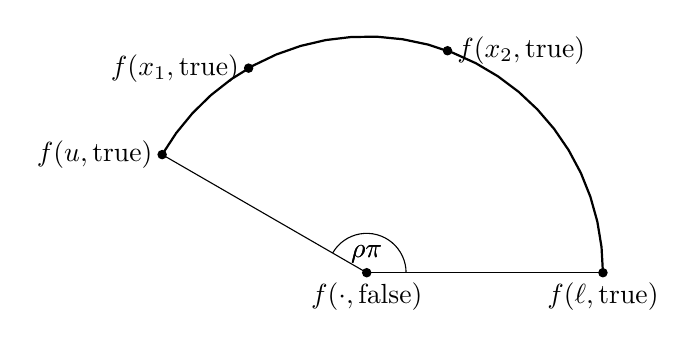
\begin{tikzpicture}

\pgfmathsetlengthmacro{\r}{3cm}
	\coordinate (O) at (0, 0);
	\coordinate (left) at ({3*cos(150)}, {3*sin(150)});

	\coordinate (right) at (\r, 0);
	\coordinate (x1) at ({3*cos(120)}, {3*sin(120)});
	\coordinate (x2) at ({3*cos(70)}, {3*sin(70)});

	% Draw big arc	
	\draw [black,thick,domain=0:150] plot ({3*cos(\x)}, {3*sin(\x)});

	\draw[fill] (left) circle (1.5pt);
	\draw (left) node[below, left] {$f(u, \textnormal{true})$};
	
	\draw[fill] (right) circle (1.5pt);
	\draw (right) node[below] {$f(\ell, \textnormal{true})$};

	\draw[fill] (O) circle (1.5pt);
	\draw (O) node[below] {$f(\cdot, \textnormal{false})$};

	\draw[fill] (x1) circle (1.5pt);
	\draw (x1) node[above, left] {$f(x_1, \textnormal{true})$};

	\draw[fill] (x2) circle (1.5pt);
	\draw (x2) node[above, right] {$f(x_2, \textnormal{true})$};
	
	% Draw little arc to denote the angle
	\draw (left) -- (O) node[above] {$\rho \pi$};
	\draw (right) -- (O) node[above] {$\rho \pi$};
	\draw [black,domain=0:150] plot ({0.5*cos(\x)}, {0.5*sin(\x)});
	
  \end{tikzpicture}
\end{center}
\caption{A demonstration of the embedding giving rise to the pseduo-metric: All points for which $\delta_i(x) =$ false are mapped to the same point.  Points for which $\delta_i(x) =$ true are mapped to a semicircle.  This embedding gives a constant distance between pairs of points which have differing values of $\delta$.  The parameter $\rho$ determines how much distance there is along the arc.}
\end{figure}
\end{document}